% !TEX root = DesignDoc.tex

\chapter{Electrical Design}
\label{chap:elecdesign}

This chapter details the electrical components used in the design, and includes logical connection diagrams.

\section{Parts List}

Both the SMP and Mecanum robots used nearly identical parts for the electrical system. This was by design to reduce the number of different parts the lab would need to keep on hand for replacements. It also simplified the build process because we were able to prototype with a single robot, rather than going through the prototyping phase for each one. The items marked with (*) varied between the SMP and Mecanum designs.

\begin{itemize}
	\item{DC Motors with Encoders (4)*}
	\item{Motor Controller(2)*}
	\item{11.1V LiPo Battery(2)}
	\item{Contactor(1)}
	\item{DC-DC Converter(1)}
	\item{Power Switch(1)}
	\item{Terminal Blocks(4)}
	\item{Odroid XU3 Lite(1)}
	\item{Wireless Router(1)}
	\item{LiDAR(1)}
	\item{ASUS(1)}
	\item{IMU(1)}
\end{itemize}

\subsection{DC Motors With Encoders}

Each robot uses four (4) Brushed DC Motors with quadrature encoders mounted on the back shaft. Both use a 42mm motor made by Shayang Ye Industrial Co., Ltd.. The Mecanum robot uses the 24:1 gear ratio, while the SMP robots use the 49:1 gear ratio. The relevant datasheets should be included with this document:

\begin{itemize}
\item{\href{run:IG42-Gear-Motor.pdf}{Motor}}
\item{\href{run:IG42-Gear-Box.pdf}{Gearbox}}
\item{\href{run:encoder-datasheet.pdf}{Encoder}}
\end{itemize}

\subsection{Motor Controller}

\subsubsection{SMP}

The SMPs each use two (2) \href{run:roboteq-motor-controller.pdf}{SDC-2130 RoboteQ motor controllers}. We never quite got the serial communication working with these guys, so they are currently still connected through USB. This is undesirable as it violates one of our requirements from Chapter \ref{chap:requirements}. I'm still not sure why the serial communication didn't work. Kudos to whoever figures out what I missed. It's probably something simple. Most problems turn out to be simple.

\subsubsection{Mecanum}

The Mecanum uses two (2) \href{run:roboclaw-motor-controller.pdf}{Roboclaw 2-15A motor controllers}. There is one odd caveat of the Roboclaw motor controllers I want to document here. The Roboclaw allows up to 8 contollers to be networked on one serial line. All of the receive (rx) pins from the motor controllers just tie together and lead to the one transmit (tx) pin on the Odroid. However, because we can't have multiple units attempting to "talk" on one transmit line, a diode is required on each individual motor controller tx pin, and a single pull-up resistor is required on the line. This diode will prevent problems with collisions, because the line can only be pulled low by the motor controllers, but it cannot be pulled high. There's some serial arbitration magic in there as well, which I don't fully understand, but I do know that without those diodes it will not work.

\subsection{Contactor}

Both robot types use one (1) \href{run:contactor.pdf}{White Rodgers 124-309 Contactor}.

\subsection{DC-DC Converter}

Both robot types use 1 (1) \href{run:Mean_Well-RSD-100B-5-datasheet.pdf}{Mean Well RSD-100B-5 DC-DC Converter}.

\subsection{Power Switch}

Both robot types use simple mechanical switches to activate the contactors. The two SMPs use key switches from Chris Supply in Rapid City. The Mecanum uses a simple throw switch I found randomly in the lab.

\subsection{Terminal Blocks}

Both robot types use terminal blocks with screw terminals to distribute power. There is a +24V unregulated and 0V unregulated in the cage. There is also a regulated set of 5V and 0V terminal blocks on the top of each robot. These terminal blocks were from Chris Supply in Rapid City.

\subsection{Odroid XU3 Lite}

Documentation on the Odroid XU3 Lite exists, but it's sort of spread out all over the Hardkernel website, so there isn't an easy way to just link to a .pdf. Sorry about that.

\subsection{Wireless router}
Each robot has a wireless router to allow connection and programming wirelessly. I stole three routers from the turtle-bots and can't remember any actual information about them other than that they worked.

\subsection{LiDAR}

There are two \href{run:HokoyuURG_Datasheet.pdf}{Hokoyu LiDAR}s currently floating between the three robots. These LiDARs are good both indoors and out, but perform best indoors.

\subsection{ASUS}

Each robot has an ASUS RGBD sensor. This allow for depth sensing as well as color vision. The ASUS also has a built-in microphone. There isn't a readily available .pdf to present with this document, so online will be your best resource.

\subsection{IMU}

The two SMP robots currently have one (1) \href{run:HokoyuURG_Datasheet.pdf}{YEI 3-Space Motion} sensors that allow them to infer their pitch, yaw, and roll, as well as measure accelerations.

%\pagebreak
\section{Wiring Diagrams}

%\subsection{Power}

\begin{figure}[h]
\centering
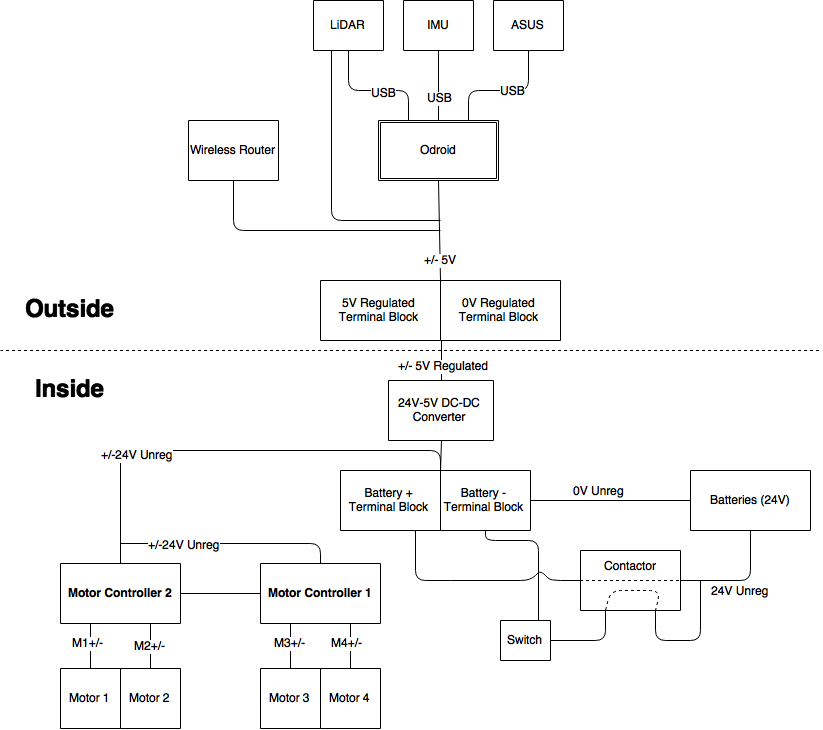
\includegraphics[width=\textwidth]{PowerDiagram.png}
\label{fig:powerdiagram}
\caption{Power Connections}
\end{figure}
%\pagebreak
%\subsection{Logic}

\begin{figure}[h]
\centering
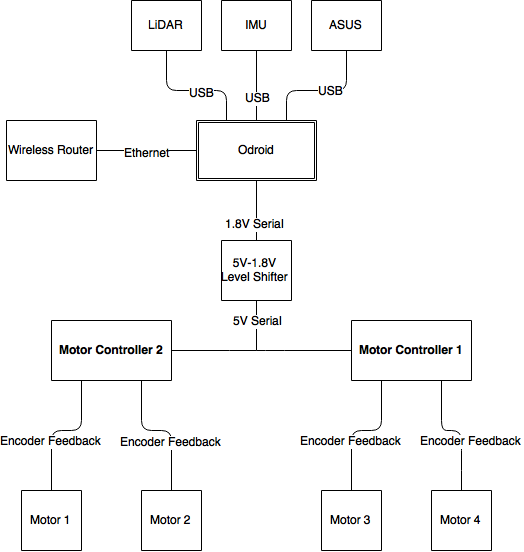
\includegraphics[width=.75\textwidth]{LogicDiagram.png}
\label{fig:logicdiagram}
\caption{Logical Connections}
\end{figure}